\documentclass[11pt]{article}
\usepackage[utf8]{inputenc}
\usepackage[T1]{fontenc}
\usepackage[spanish,es-tabla]{babel} % idiomas (uno o varios)

\usepackage[left = 2.25cm, right = 2.25cm, top=1.5cm, bottom = 1.5cm]{geometry}
\usepackage{mathtools} % símbolos extensibles (contiene amsmath)
\usepackage{amssymb} % símbolos matemáticos
\usepackage{mathrsfs} % para usar \mathscr{}
\usepackage{physics} % notación de Dirac
\usepackage{tensor} % índices en cualquier lado

\usepackage{booktabs} % tablas
\usepackage[bookmarks = true, colorlinks=true, linkcolor = black, citecolor = black, menucolor = black, urlcolor = black]{hyperref} % para referencias cruzadas
\usepackage[table]{xcolor} % colores (incluye colortbl la cargarlo con table)
\usepackage{tcolorbox} % cajas de colores con titulo

\usepackage{float} % para figuras (las fija, [H], ...)
\usepackage{graphicx} % para figuras
\usepackage{caption} % pie de foto
\usepackage{subcaption} % pie de ''subfoto''


\selectlanguage{spanish}
\renewcommand{\theenumi}{\roman{enumi}}
\renewcommand{\thefigure}{\Roman{figure}} 
\newcommand\diagram[2]{\schema{\schemabox{#1}}{\schemabox{#2}}}
\usepackage{comment}

\begin{document}

\subsubsection*{Ejercicio 1}

\begin{table}[H]
\centering
\begin{tabular}{ccccc}
\toprule
Observación & $X_1$ & $X_2$ & Y & $\alpha$ \\
\toprule
1 & 2 & 6 & 1 & 0 \\
2 & 4 & 3 & 1 & 1 \\
3 & 4 & 4 & 1 & 0.3333 \\
4 & 4 & 6 & 1 & 0 \\
5 & 6 & 3 & 1 & 1 \\
6 & 7 & 7 & 1 & 0.1667 \\
7 & 8 & 4 & 1 & 1 \\
8 & 9 & 8 & 1 & 1 \\
9 & 2 & 1 & -1 & 1 \\
10 & 6 & 2 & -1 & 0.5 \\
11 & 7 & 4 & -1 & 1 \\
12 & 8 & 8 & -1 & 1 \\
13 & 9 & 1 & -1 & 0 \\
14 & 10 & 3 & -1 & 0 \\
15 & 10 & 6 & -1 & 1 \\
16 & 12 & 4 & -1 & 0 \\
\toprule
\end{tabular}
\caption{Dataset con valores de $\alpha$}
\label{tab:dataset_alpha}
\end{table}

\begin{enumerate}
\item \textbf{Indica cuáles son los vectores de soporte y cuáles de ellos están en el límite del margen.}
\begin{itemize}
\item Vectores de soporte: observaciones 2, 3, 5, 6, 7, 8, 9, 10, 11, 12, 15.
\item Vectores de soporte en el límite del margen: observaciones 3, 6, 10.
\end{itemize}
\item \textbf{Indica cuáles son los coeficientes del hiperplano ($\beta$ y $\beta_0$) y el valor de M.}
\begin{itemize}
\item Coeficientes del hiperplano: $\beta = (-0.5, 0.5)$, $\beta_0 = 1$
\item Valor de $M$: $\sqrt{2} \approx 1.4142$
\end{itemize}
\item \textbf{Indica los valores de $\varepsilon_i$ y las observaciones incorrectamente clasificadas.}
\begin{table}[H]
\centering
\begin{tabular}{cccccc}
\toprule
Observación & $X_1$ & $X_2$ & Y & $\alpha$ & $\varepsilon_i$ \\
\toprule
1 & 2 & 6 & 1 & 0 & 0 \\
2 & 4 & 3 & 1 & 1 & 0.5 \\
3 & 4 & 4 & 1 & 0.3333 & 0 \\
4 & 4 & 6 & 1 & 0 & 0 \\
\textcolor{red}{5} & \textcolor{red}{6} & \textcolor{red}{3} & \textcolor{red}{1} & \textcolor{red}{1} & \textcolor{red}{1.5} \\
6 & 7 & 7 & 1 & 0.1667 & 0 \\
\textcolor{red}{7} & \textcolor{red}{8} & \textcolor{red}{4} & \textcolor{red}{1} & \textcolor{red}{1} & \textcolor{red}{2} \\
8 & 9 & 8 & 1 & 1 & 0.5 \\
\textcolor{red}{9} & \textcolor{red}{2} & \textcolor{red}{1} & \textcolor{red}{-1} & \textcolor{red}{1} & \textcolor{red}{1.5} \\
10 & 6 & 2 & -1 & 0.5 & 0 \\
11 & 7 & 4 & -1 & 1 & 0.5 \\
\textcolor{red}{12} & \textcolor{red}{8} & \textcolor{red}{8} & \textcolor{red}{-1} & \textcolor{red}{1} & \textcolor{red}{2} \\
13 & 9 & 1 & -1 & 0 & 0 \\
14 & 10 & 3 & -1 & 0 & 0 \\
15 & 10 & 6 & -1 & 1 & 0 \\
16 & 12 & 4 & -1 & 0 & 0 \\
\toprule
\end{tabular}
\caption{Valores de $\varepsilon_i$ para cada observación. En rojo, las observaciones mal clasificadas.}
\label{tab:2}
\end{table}
\end{enumerate}


\subsubsection*{Ejercicio 2}

\begin{itemize}
    \item \textbf{Menor error de validación cruzada, su desviación estándar y valor de los hiperparámetros:} 
    \begin{itemize}
    \item Kernel lineal: $\Delta = 0.234146$, $\sigma = 0.01123$, $\text{param\_C} = 100000$.
    \item Kernel polinómico: $\Delta = 0.220728$, $\sigma = 0.037121$, $\text{param\_C} = 10000$, $\text{param\_degree} = 3$.
    \item Kernel radial: $\Delta = 0.195616$, $\sigma = 0.021161$, $\text{param\_C} = 1$, $\text{param\_gamma} = 1$.
    \end{itemize}
    \item \textbf{Error de test para los hiperparámetros de validación cruzada:} 
    \begin{itemize}
    \item Kernel lineal: $\Delta = 0.22$
    \item Kernel polinómico: $\Delta = 0.233333$
    \item Kernel radial: $\Delta = 0.226667$
    \end{itemize}
\end{itemize}


\begin{figure}[h]
\centering
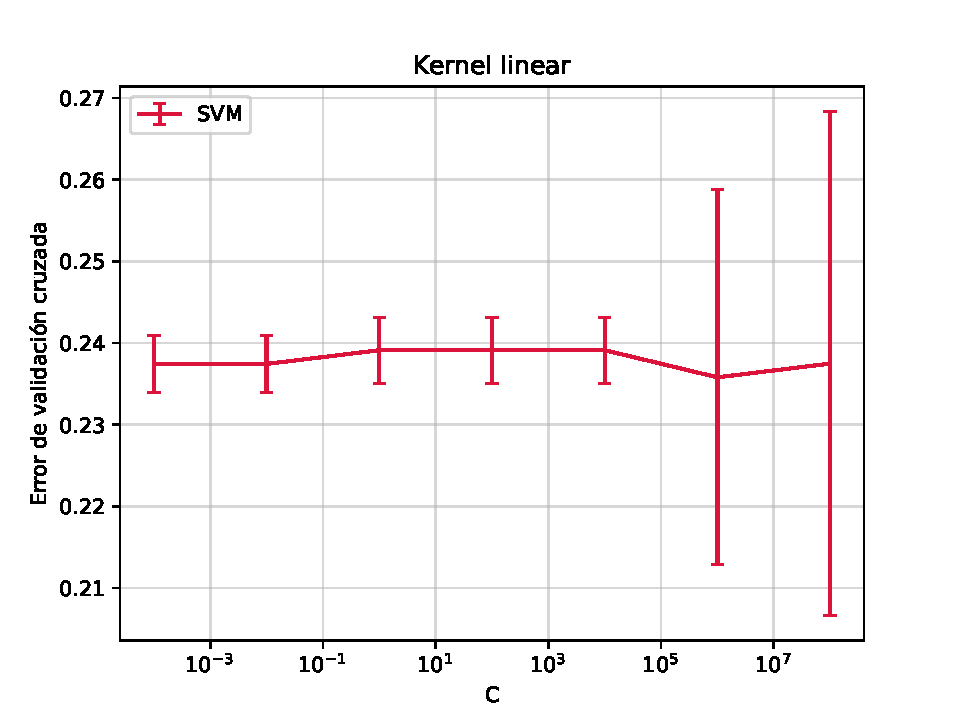
\includegraphics[width=0.75\textwidth]{fotos/lineal_gg.pdf}
\caption{Ejercicio 2: error de validación cruzada en datos de validación para el kernel lineal (exploración de grano grueso).}
\end{figure}

\begin{figure}[h]
\centering
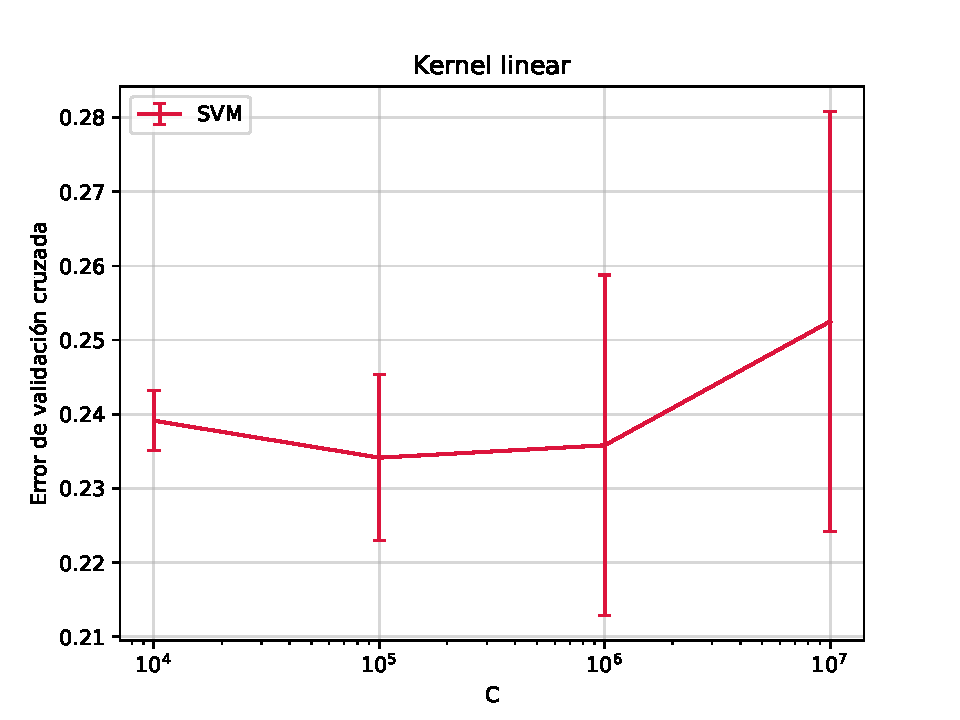
\includegraphics[width=0.75\textwidth]{fotos/lineal_gf.pdf}
\caption{Ejercicio 2: error de validación cruzada en datos de validación para el kernel lineal (exploración de grano fino).}
\end{figure}

\begin{figure}[h]
\centering
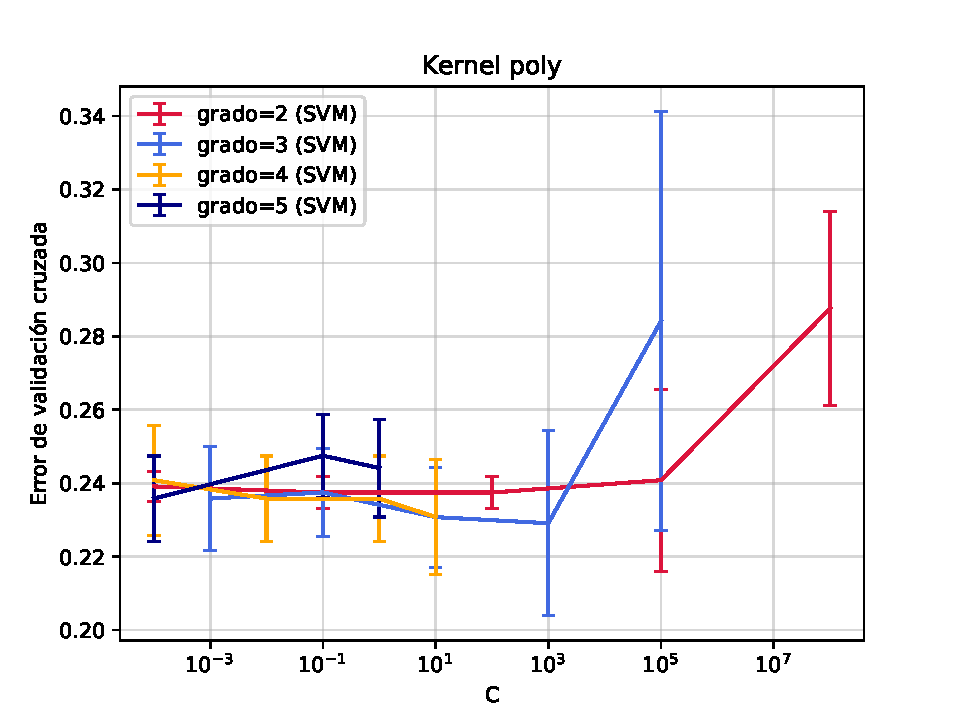
\includegraphics[width=0.75\textwidth]{fotos/poly_gg.pdf}
\caption{Ejercicio 2: error de validación cruzada en datos de validación para el kernel polinómico (exploración de grano grueso).}
\end{figure}

\begin{figure}[h]
\centering
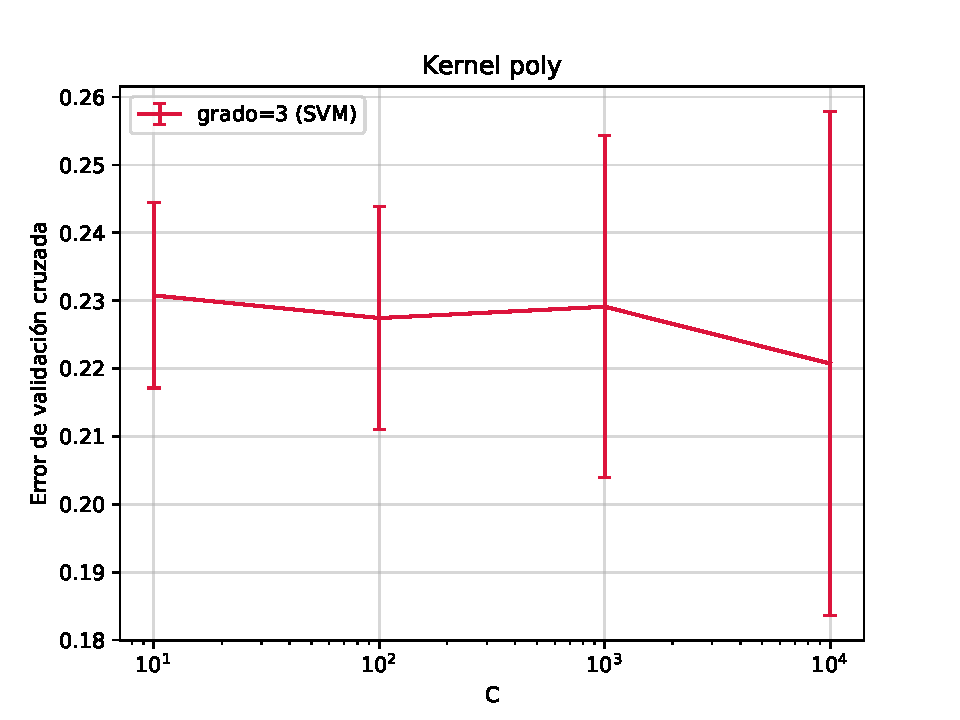
\includegraphics[width=0.75\textwidth]{fotos/poly_gf.pdf}
\caption{Ejercicio 2: error de validación cruzada en datos de validación para el kernel polinómico (exploración de grano fino).}
\end{figure}

\begin{figure}[h]
\centering
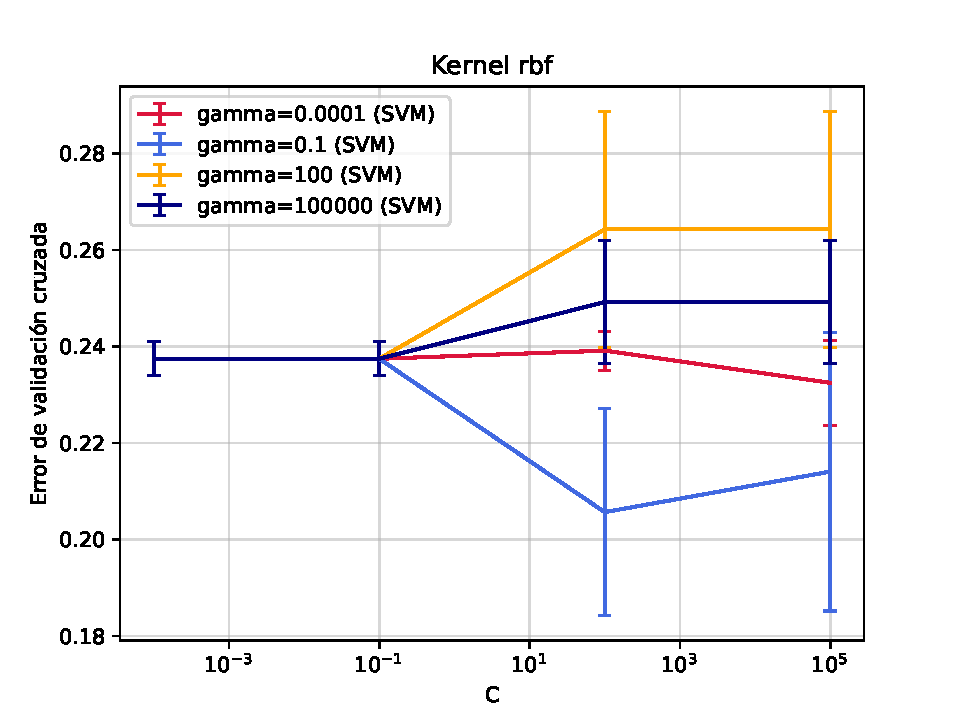
\includegraphics[width=0.75\textwidth]{fotos/rbf_gg.pdf}
\caption{Ejercicio 2: error de validación cruzada en datos de validación para el kernel radial (exploración de grano grueso).}
\end{figure}

\begin{figure}[h]
\centering
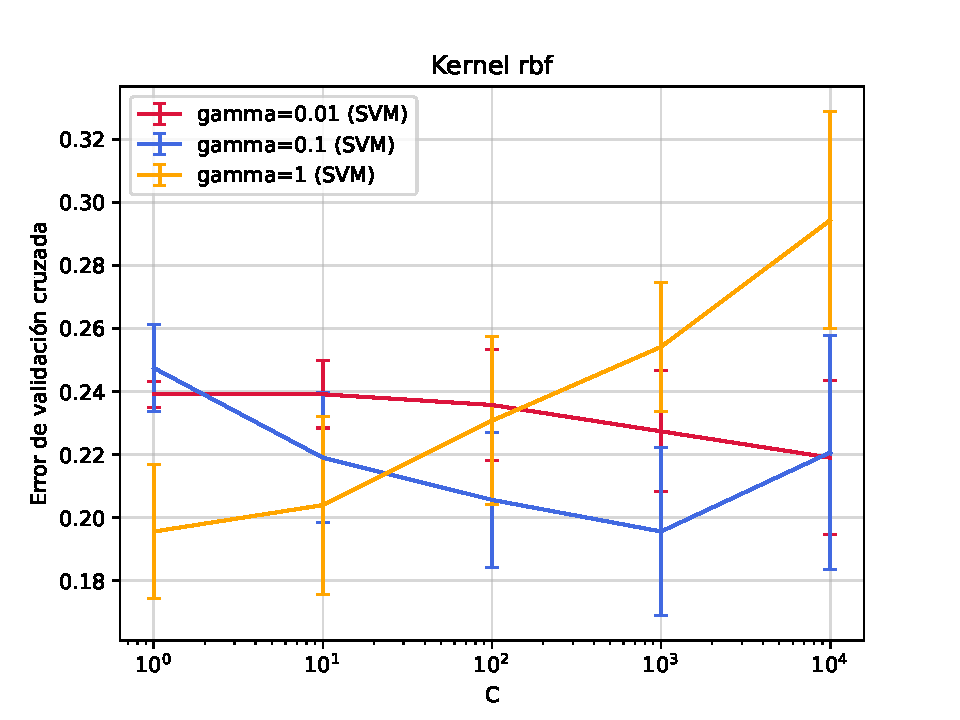
\includegraphics[width=0.75\textwidth]{fotos/radial_gf.pdf}
\caption{Ejercicio 2: error de validación cruzada en datos de validación para el kernel radial (exploración de grano fino).}
\end{figure}

\begin{figure}[h]
\centering
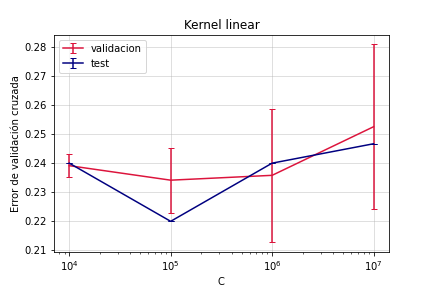
\includegraphics[width=0.75\textwidth]{fotos/linealTest.png}
\caption{Ejercicio 2: error de validación cruzada en datos de validación frente al mismo error en datos de test para el kernel lineal.}
\end{figure}

\begin{figure}[h]
\centering
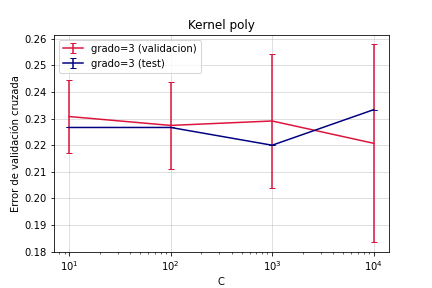
\includegraphics[width=0.75\textwidth]{fotos/polyTest.png}
\caption{Ejercicio 2: error de validación cruzada en datos de validación frente al mismo error en datos de test para el kernel polinómico de grado 3.}
\end{figure}

\begin{figure}[h]
\centering
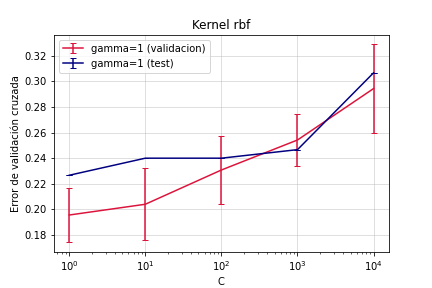
\includegraphics[width=0.75\textwidth]{fotos/radialTest.png}
\caption{Ejercicio 2: error de validación cruzada en datos de validación frente al mismo error en datos de test para el kernel radial.}
\end{figure}

\end{document}
